\documentclass{article}

% packages
\usepackage[a4paper, margin=2.2cm]{geometry}
\usepackage{multicol}
\usepackage[utf8]{inputenc}
\usepackage[english]{babel}
\usepackage{minted}
\usepackage{tikz}
\usepackage{pgfplots}
\usepackage{parskip}
\usepackage{amsmath}
\usepackage{xcolor}
\usepackage[justification=centering, margin=1.6cm]{caption}
\usepackage{graphics}

\pgfplotsset{compat=1.16}

\newlength\figurewidth
\newlength\figureheight
\setlength\figurewidth{0.3\textwidth}
\setlength\figureheight{0.3\textwidth}

\begin{document}

    \begin{titlepage}
        \begin{center}
            \vspace*{2cm}
            
            {\huge \textbf{xCore-200 Cellular Automaton Farm}}
            
            \vspace{0.5cm}
            
            {\Large COMS20001 Concurrent Computing CW1}
            
            \vspace{0.5cm}
            
            {\large Team 6}
            
            \vspace{1cm}
            
            \hspace*{1cm} {\Large \textbf{Ruairi Fox}} \hfill {\Large \textbf{Liam Dalgarno}} \hspace*{1cm} \\~\\[-0.5em]
            \hspace*{1cm} MEng. Computer Science \hfill MEng. Computer Science  \hspace*{1cm} \\~\\[-1em]
            \hspace*{1cm} rf17160@bristol.ac.uk  \hfill ld17285@bristol.ac.uk  \hspace*{1cm} 
            
            \vspace{1cm}
            
            {\large \today}
        \end{center}
    \end{titlepage}

    \section{Functionality and Design}
    1 Page Max: Outline what functionality you have implemented, which problems you have solved with your implementation and how your program is designed to solve the problems efficiently and effectively
    \pagebreak

    \section{Tests and Experiments}
    
    The main factors which contribute to the success and shortcomings of our system are the choice of architecture, bit packing and the algorithm for evolving the game. These factors together allow us to process images larger than \verb|1024x1024|. We tested our system in multiple ways, such as:
    
    \begin{itemize}
        \setlength\itemsep{-0.2\baselineskip}
        \item Comparing two iterations of a \verb|32x32| image to another implementation of the Game of Life. (Figure \ref{fig:test32})
        \item Examining some sample generations of a \verb|1024x1024| image starting from a straight line. (Figure \ref{fig:test1024})
        \item Varying our system parameters to see how it impacts the processing time. (Figure \ref{fig:agt} and Section \ref{analysis})
    \end{itemize}
    
    \begin{figure}[h]
        \begin{center}
            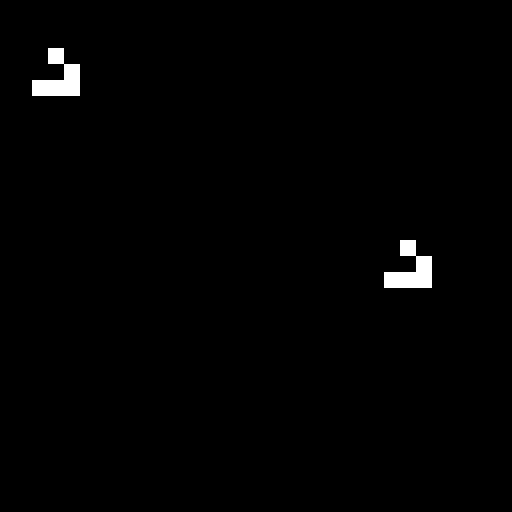
\includegraphics[width=0.15\textwidth]{test32.png}
            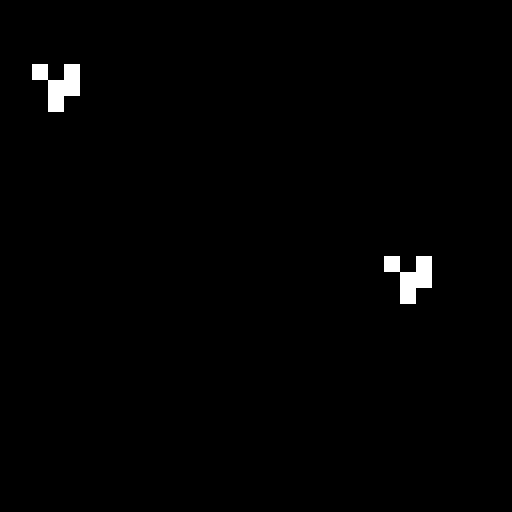
\includegraphics[width=0.15\textwidth]{testout32-1.png}
            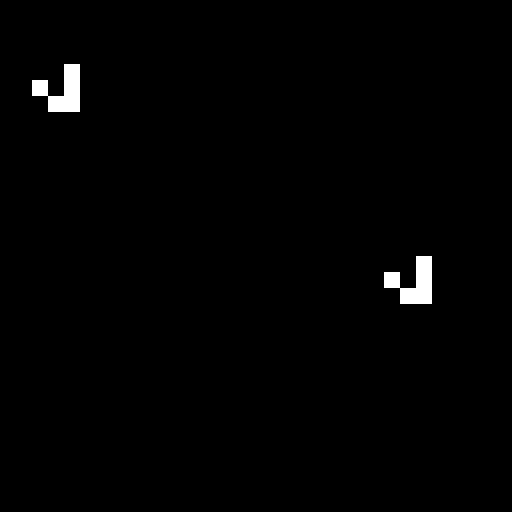
\includegraphics[width=0.15\textwidth]{testout32-2.png}
            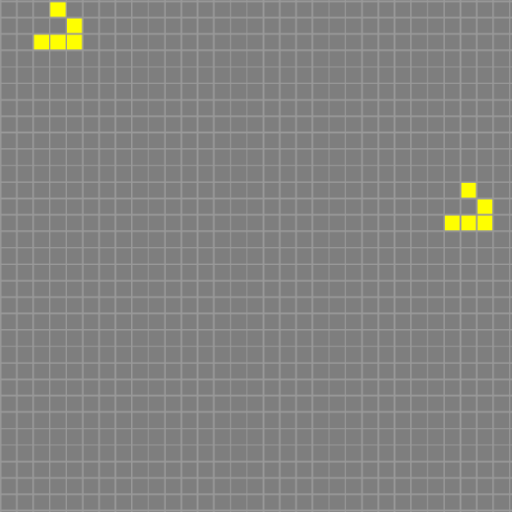
\includegraphics[width=0.15\textwidth]{verify32.png}
            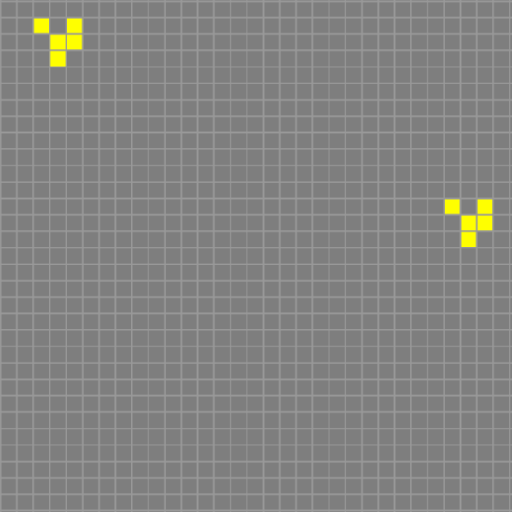
\includegraphics[width=0.15\textwidth]{verify32-1.png}
            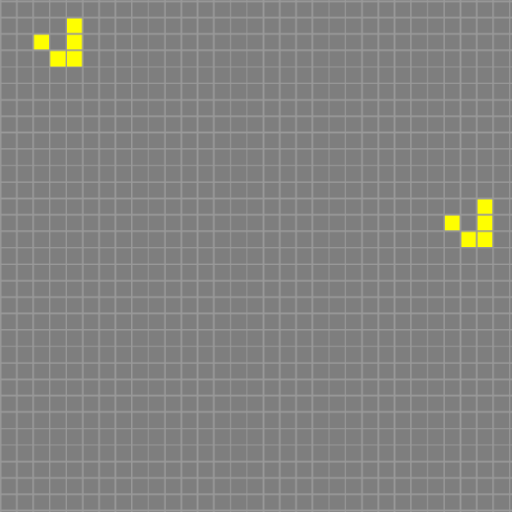
\includegraphics[width=0.15\textwidth]{verify32-2.png}
            \caption{State following 2 iterations of a \texttt{32x32} image. \\ Left: our system; Right: \texttt{https://bitstorm.org/gameoflife/}}
            \label{fig:test32}
        \end{center}
    \end{figure}

    \begin{figure}[h]
        \begin{center}
            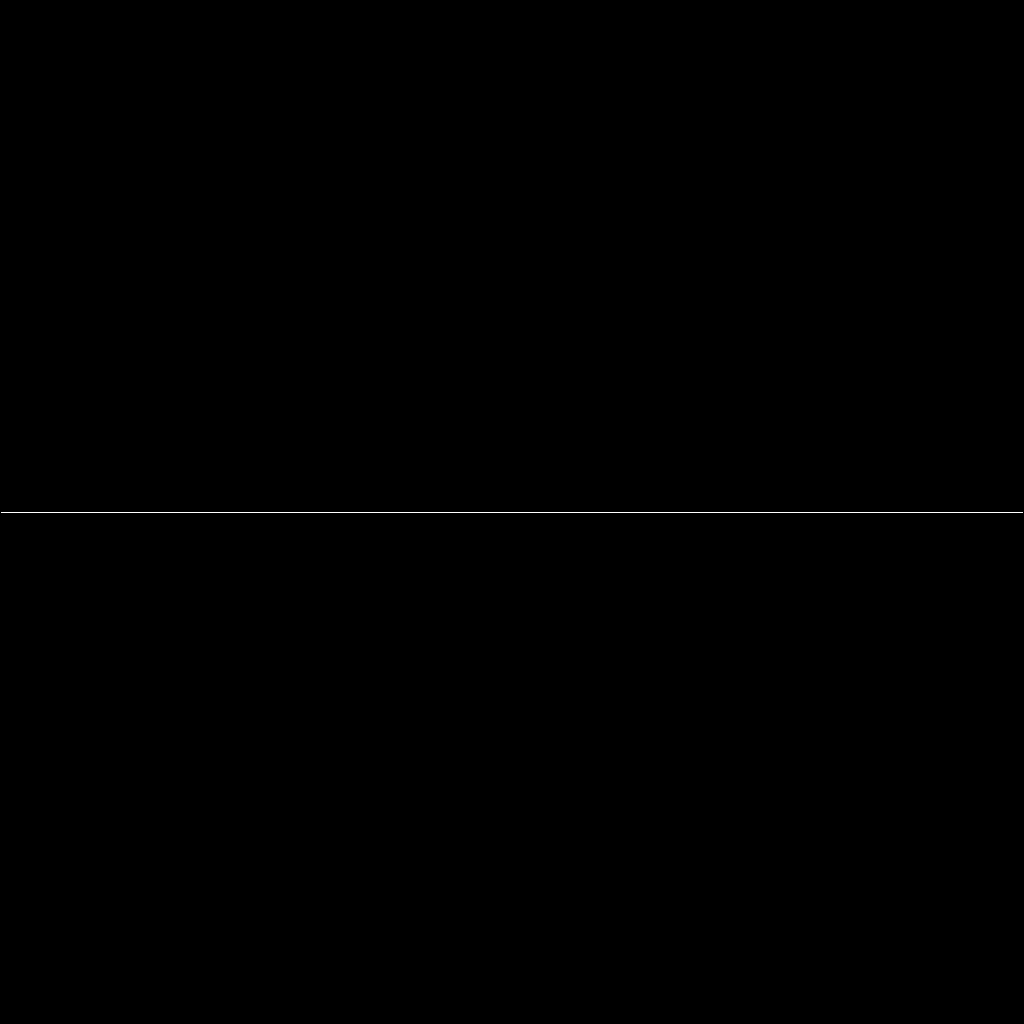
\includegraphics[width=0.2\textwidth]{test1024.png}
            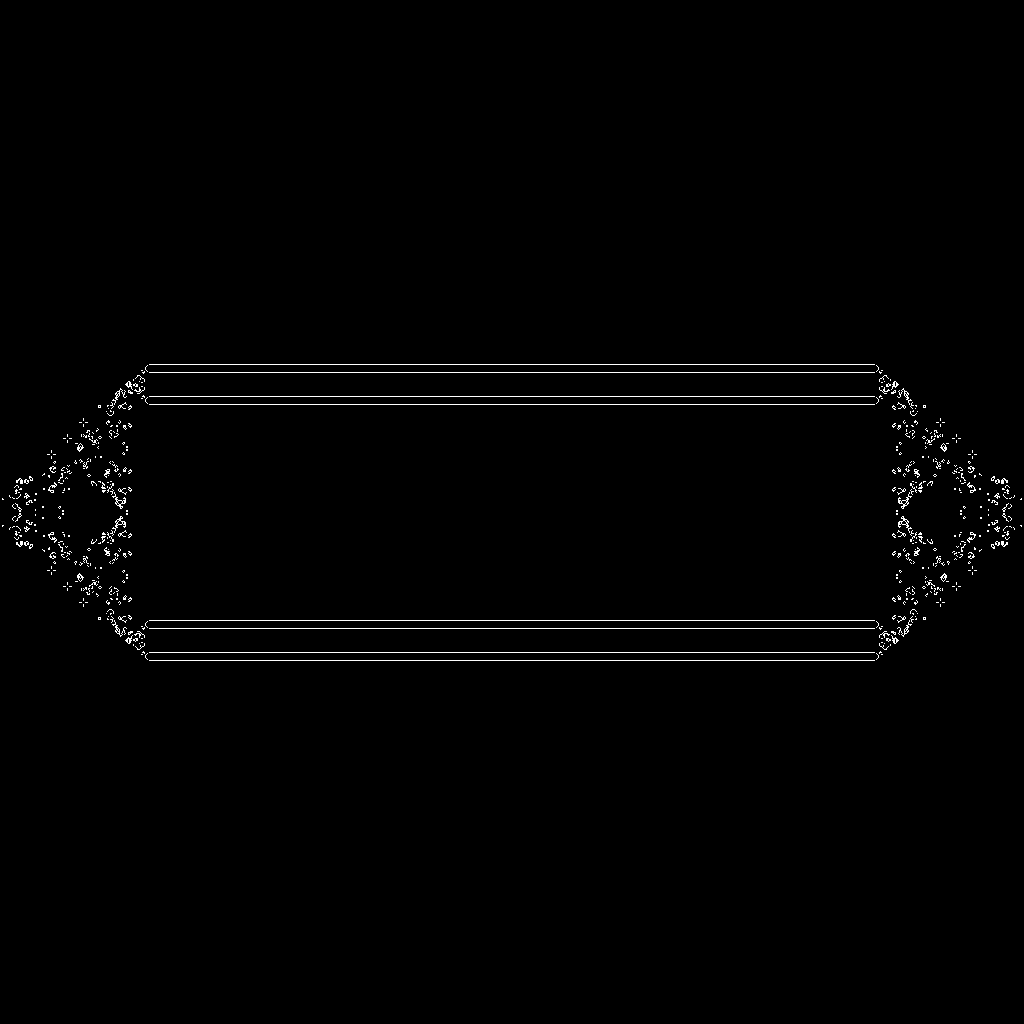
\includegraphics[width=0.2\textwidth]{testout1024-1.png}
            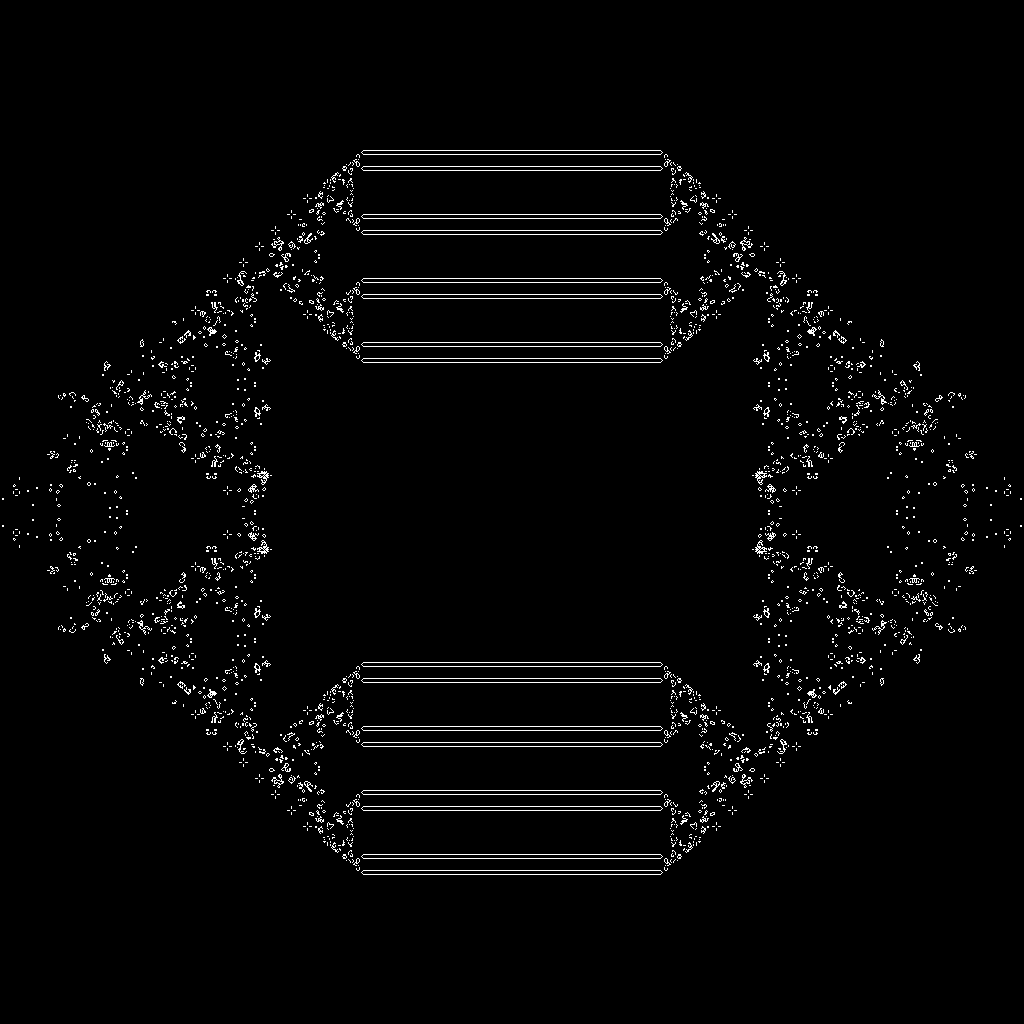
\includegraphics[width=0.2\textwidth]{testout1024-2.png}
            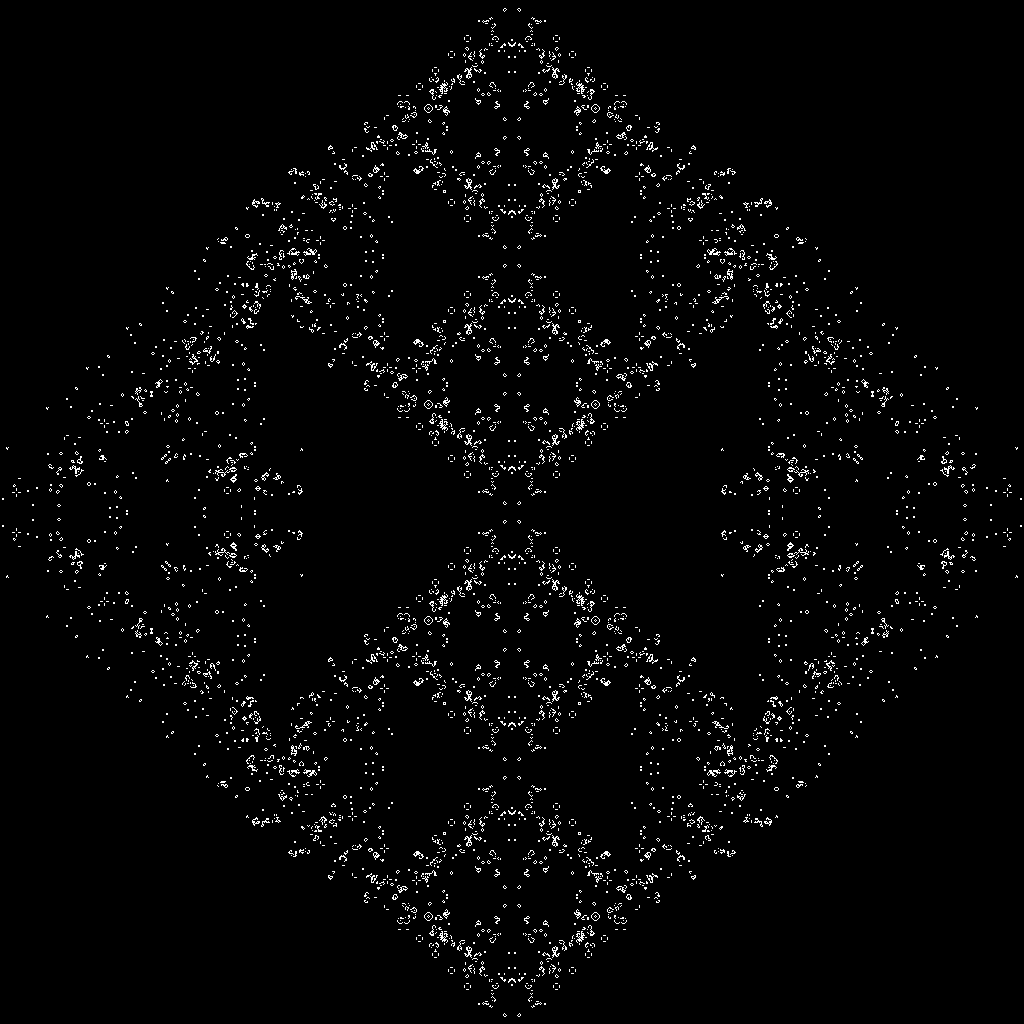
\includegraphics[width=0.2\textwidth]{testout1024-3.png}
            \caption{Example generations of a \texttt{1024x1024} image, beginning from a straight line.}
            \label{fig:test1024}
        \end{center}
    \end{figure}
    
    \subsection{Architecture and the Distributor}
    
    Without an effective memory distribution and architecture, our system was unable to process images larger than \verb|512x512|. We chose to make the \verb|distributor| `organise' the cell data from \verb|data_in| and send it to the correct worker a packet at a time. Without this approach, the \verb|distributor| would need to store the initial state of the board, which would be useless after the first generation, and would take up $1024 \cdot 32 \cdot 4 = 131072$KB for a \verb|1024x1024| image. 
    
    Since the \verb|distributor| is not using memory redundantly, the tiles use approximately the same amount of memory. Therefore, we can implement storing the board evenly across both tiles to effectively double the space we can use for the board. Each worker communicates with their `neighbour' workers based on their position in the image (Figure \ref{fig:architecture}) to swap their overlapping rows. This allows the workers to be `isolated' and work on their respective portion of the image in parallel.
    
    \begin{figure}[h]
        \begin{center}
            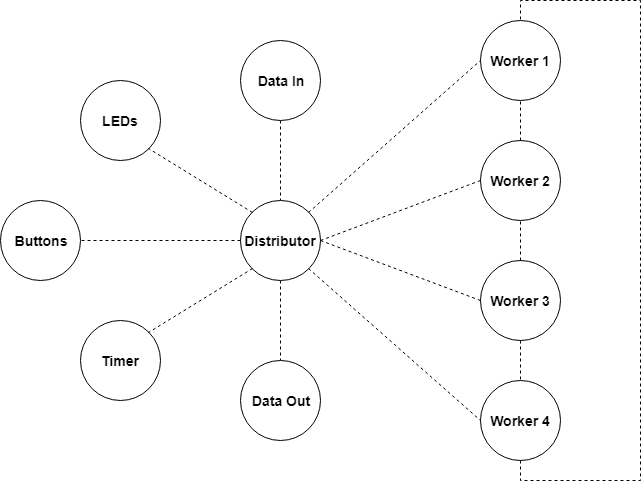
\includegraphics[width=0.4\textwidth]{architecture.png}
            \caption{High-level channel architecture.}
            \label{fig:architecture}
        \end{center}
    \end{figure}


    \subsection{Bit Packing}

    Packing 32 cells into a single 32-bit integer massively improves the performance of the system, but does bring a small downside. The memory usage is reduced by a factor of 8 since each cell is represented using 1 bit rather than 8, allowing for larger boards in memory. Channel congestion however, is reduced by a factor of 32 since we can send 32 cells in one message. This reduces waiting times for channel communication, and therefore increases processing speed. A downside of bit packing is that our system is no longer compatible with images where the width is not a multiple of 32: the algorithm for evolving the generation relies on the packet being full. (Section \ref{evolution})
    
    \begin{figure}[h]
        \hspace{-0.9cm}
\begin{minipage}{0.45\textwidth}
    \begin{minted}[fontsize=\footnotesize]{C}
        uint32_t pack(uchar bits[32]) {
            uint32_t packed = 0;
            for (uchar i = 0; i < 32; i++) {
                packed |= (uint32_t) (bits[i] >> 7) << (31 - i);
            }
            return packed;
        }
    \end{minted}
\end{minipage}
\hspace{0.4cm}
\begin{minipage}{0.45\textwidth}
    \begin{minted}[fontsize=\footnotesize]{C}
        void unpack(uchar result[32], uint32_t packed) {
            for (uchar i = 0; i < 32; i++) {
                result[i] = ((packed >> (31 - i)) & 0x1) * 255;
                }
            }
        }
    \end{minted}
\end{minipage}
        \caption{Bit packing code}
        \label{fig:bitpack}
    \end{figure}

    \subsection{Evolution} \label{evolution}

    The algorithm for evolving the board carries two `quirks' with it to save memory. Firstly, the algorithm operates solely on the packed cells and never unpacks them. Rather, it uses bit shifting and modular arithmetic to calculate the number of neighbours a cell has. 

    \begin{figure}[h]
        \begin{minted}[fontsize=\footnotesize]{C}
// l, c, r represent the shifts to get the neighbouring cell bits
// l_pack and r_pack are the left and right packed bits
// they're usually the same unless the current bit is on the edge of the pack
unsigned char l = mod(-i, 32), c = 31 - i, r = i == 31 ? 31 : 30 - i;
unsigned char l_pack = i == 0 ? mod(x - 1, PACKED_WD) : x;
unsigned char r_pack = i == 31 ? mod(x + 1, PACKED_WD) : x;
unsigned char neighbours = ((cells[u_row][l_pack] >> l) & 0x1) 
                         + ((cells[u_row][x]      >> c) & 0x1) 
                         + ((cells[u_row][r_pack] >> r) & 0x1)
                         + ((cells[y][l_pack]     >> l) & 0x1)
                         + ((cells[y][r_pack]     >> r) & 0x1)
                         + ((cells[d_row][l_pack] >> l) & 0x1) 
                         + ((cells[d_row][x]      >> c) & 0x1) 
                         + ((cells[d_row][r_pack] >> r) & 0x1);
\end{minted}
        \caption{Algorithm for calculating the current cell's neighbour count.}
        \label{fig:evolve}
    \end{figure}

    Secondly, there is only one copy of the board which stores both the state of the current generation and the next. This exploits the fact that once a row is processed, the row above is redundant, so we can overwrite it with the new processed row. Of course, the downside of this approach is that the next generation is shifted upwards by one row. Its necessary to shift every row back down, which could impact performance..

    \begin{figure}[h]
        \begin{center}
            \begin{alignat*}{3}
    &\big[0101\dots1110\big]         &{}                                                                                     &\big[\textcolor{green!60!black}{0100\dots0010}\big] \\
    &\big[\textcolor{cyan!75!black}{0111\dots0110}\big] \mapsto &\big[\textcolor{green!60!black}{0100\dots0010}\big] \mapsto &\big[\textcolor{cyan!75!black}{0111\dots0110}\big] \\
    &\big[1100\dots1000\big]         &{}                                                                                     &\big[1100\dots1000\big] 
\end{alignat*}
            \begin{minipage}{0.5\textwidth}
    \begin{minted}[fontsize=\footnotesize]{C}
    // ...
    for (short i = 0; i < PACKED_WD; i++) {
        cells[y - 1][i] = processed[i];
    }
    // ...
    // shift cells back down
    for (short y = WORKER_ROWS; y > 0; y--) {
        for (short x = 0; x < PACKED_WD; x++) {
            cells[y][x] = cells[y - 1][x];
        }
    }
    \end{minted}
\end{minipage}
            \caption{Processing the current row and placing it in the row above. \\ Green: next generation row; Blue: current generation row.}
            \label{fig:rows}
        \end{center}
    \end{figure}

    \pagebreak

    % ?? is a placeholder for a future citation :)
    \section{Critical Analysis} \label{analysis}

    \begin{figure}[h]
        \begin{center}
            {\small
\begin{tabular}{|c|c|c|c|c|}
    \hline Size & AGT2 (ms) & AGT4 (ms) & AGT8 (ms) \\
    \hline \verb|64x64| & 11.64 & 11.65 & 11.64 \\
    \verb|128x128| & 39.88 & 20.12 & 11.64 \\
    \verb|256x256| & 161.89 & 80.77 & 40.31 \\
    \verb|512x512| & 621.29 & 313.71 & 157.88 \\
    \verb|1024x1024| & 2472.33 & 1250.44 & 622.59 \\
    \hline
\end{tabular}}
            \caption{The effect of increasing worker count and size of image on Average Generation Time.}
            \label{fig:agt}
        \end{center}
    \end{figure}

    Our system can maximally process approximately \verb|3,240,000| cells (a \verb|1800x1800| image) across 2-8 workers. 
\end{document}